
% Activate the appendix
% from now on sections are numerated with capital letters
\appendix

\section{Byte repacking in GNU Radio}
\label{sec:appendix_a}
The \textit{Integer 8} or \textit{Byte} data type is often used in GNU Radio. Special attention is needed for the number of bits used in the byte. 
Sometimes, a byte stream carries less than 8 bits of data per byte and it is called "unpacked". When $X$ bits per byte are used for data, only the $X$ least significant bits can be non-zero and these bits are called the significant bits. The other $8-X$ bits are always zero. As a consequence, the \textit{rate} of the stream will be changed. For every incoming byte, $8/X$ output bytes are generated. \medskip

Some blocks output data with 8 significant bits per byte, while others expect a data stream with for example 2 bits per byte. In that case, the byte stream has to be repacked. Several blocks exist for this purpose, but the most universal blocks is the Repack Bits block. The block can repack bits in a MSB-first or LSB-first way, and adapt a tag value to the new number of output bytes.

\paragraph*{LSB-first repacking}
LSB-first repacking means that the least significant bit of the input byte is read first, and the output bytes are filled LSB-first. When the output byte has $X$ filled bytes, the next byte will be filled.
\begin{figure}[H]
    \centering
    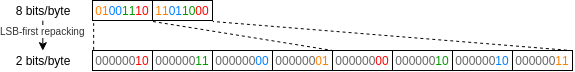
\includegraphics[width=1\textwidth]{img_packets/repacking_lsb.png}
    \caption{Unpacking example for LSB-first, with $X = 2$}
    \label{fig:repacking_lsb}
\end{figure}

\paragraph*{MSB-first repacking}
MSB-first repacking means that the most significant bit of the input byte is read first, and most significant bit of the output byte is filled first.
\begin{figure}[H]
    \centering
    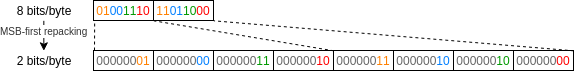
\includegraphics[width=1\textwidth]{img_packets/repacking_msb.png}
    \caption{Unpacking example for MSB-first}
    \label{fig:repacking_msb}
\end{figure}